% Giacomo Petrillo
% lezione di Morello

\begin{definition}[Covarianza]
	Date due variabili, si chiama \emph{covarianza} il valore di aspettazione
	\begin{equation*}
		\sigma_{xy} \is E[(x-\langle x\rangle)(y-\langle y\rangle)].
	\end{equation*}
	Le variabili si dicono \emph{scorrelate} o \emph{correlate} se rispettivamente la covarianza è nulla o non nulla.
\end{definition}

Si verifica immediatamente che due variabili indipendenti sono scorrelate, ma non vale il viceversa.
Prendiamo $y=x^2$. Le variabili $x$ e $y$ sono ovviamente dipendenti, ma
\begin{equation*}
	\sigma_{xy} = E[(x-\langle x\rangle)(y-\langle y\rangle)] = E[xy] - \langle x\rangle\langle y\rangle = E[x^3] - \langle x\rangle\langle y\rangle
\end{equation*}
quindi basta scegliere una distribuzione pari per $x$ affinché siano scorrelate.

\begin{exercise}
	Qual è la probabilità che, lanciando $n$ dadi, il massimo dei valori ottenuti sia $c$?
\end{exercise}

\begin{solution*}
	Vogliamo calcolare
	\begin{equation*}
		P(\max(x_1,\dots,x_n) = c).
	\end{equation*}
	Consideriamo la probabilità come distribuzione di $\max(x_i)$ e calcoliamo la cumulante:
	\begin{equation*}
		P(\max(x_i) \le c) = P\left(\bigwedge_i(x_i \le c)\right) = \prod_i P(x_i \le c) = \left (\frac c6 \right)^n.
	\end{equation*}
	Con una ``derivata discreta'' riotteniamo la distribuzione dalla cumulante:
	\begin{align*}
		&\phantom{{}={}} P(\max(x_i) = c) = \\
		&= P(\max(x_i) \le c) - P(\max(x_i) \le c-1) = \\
		&= \left (\frac c6 \right)^n - \left (\frac {c-1}6 \right)^n.
	\end{align*}
\end{solution*}

\begin{figure}
	\centering
	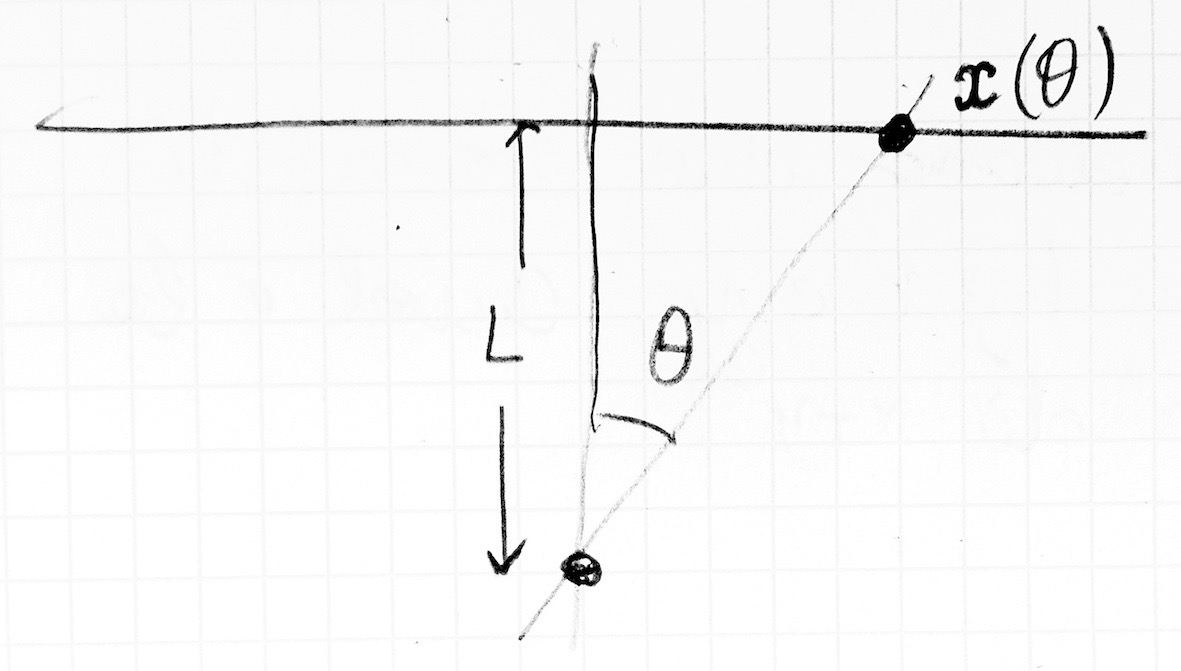
\includegraphics[width=5cm]{mitragliatrice}
	\caption{\label{fig:mitr} Una mitragliatrice spara con mira casuale contro un muro.}
\end{figure}
Considerare \autoref{fig:mitr}. $\theta$ ha una probabilità uniforme in $\left(-\frac\pi2,\frac\pi2\right)$, calcoliamo la pdf di $x(\theta)$:
\begin{align*}
	x(\theta) &= L \tan\theta \rightarrow \frac{\de x}{\de\theta} = \frac L {\cos^2\theta}, \\
	p(x) &= \frac1\pi \frac{\cos^2\theta} L = \frac1\pi\frac1{L(1+\tan^2\theta)} = \frac1{L\pi}\frac1{1+\left(\frac xL\right)^2}.
\end{align*}
La pdf che abbiamo ottenuto si chiama \emph{Cauchy}, è identica alla Breit-Wigner
\begin{equation*}
	\frac1\pi \frac {\frac\Gamma2} {\left(\frac\Gamma2\right)^2 + (x-x_0)^2}.
\end{equation*}
La distribuzione di Cauchy non ammette momenti dispari, perché l'integrale
\begin{equation*}
	\int_{-\infty}^\infty \de x\,\frac {x^n} {1+x^2}
\end{equation*}
non esiste; lo si vede dal fatto che gli integrali parziali $\int_{0}^\infty$ e $\int_{-\infty}^{0}$ divergono con segno opposto per $n \ge 1$ e dispari, quindi facendo il limite in modo diverso cambia il risultato.
Invece i momenti pari divergono, quindi la varianza rispetto a~0 (la media non esiste) è infinita.

\begin{exercise}[Somma di variabili]
	Date due variabili indipendenti $x$ e $y$, qual è la pdf di $x+y$?
\end{exercise}

\begin{solution*}
	Formalmente dobbiamo calcolare la pdf della statistica $\fundef[s]{\R^2}\R$,
	$s(x,y)=x+y$.
	Per usare il jacobiano nel cambio di variabili estendiamo $s$ aggiungendo una dimensione:
	\begin{align*}
		\mathbf s(x,y) &= \left(\begin{matrix}
			x+y \\
			y
		\end{matrix} \right) \\
		J = \frac{\partial\mathbf s}{\partial(x,y)} &= \det\left(\begin{matrix}
			1 & 1 \\
			0 & 1
		\end{matrix}\right) = 1 \\
		\implies p(\mathbf s) &= p(x,y) = p_x(x)p_y(y).
	\end{align*}
	Per ricavare la componente che ci interessa marginalizziamo:
	\begin{align*}
		p(s_1) &= \int \de s_2\, p(\mathbf s) = \\
		&= \int \de y\, p_y(y) p_x(s_1 - y) = p_x \star p_y (s_1),
	\end{align*}
	dove $\star$ indica la convoluzione.
	Avremmo potuto scrivere intuitivamente l'integrale in questo modo:
	\begin{align*}
		p(s) &= \int\limits_{x+y = s} \de x\de y\, p_x(x) p_y(y) = \\
		&= \int \de x\de y\, p_x(x) p_y(y) \delta(s - x - y) = \\
		&= \int \de x\, p_x(x) p_y(s-x).
	\end{align*}
\end{solution*}

\begin{exercise}[Prodotto e rapporto di variabili]
	Date $x$ e $y$ indipendenti calcolare le pdf di $xy$ e $\frac xy$.
\end{exercise}

\begin{solution}
	\begin{description}
		\item[Prodotto]
			$\begin{aligned}[t]
				p(s) &= \int\limits_{xy=s} \de x\de y\, p_x(x) p_y(y) = \\
				&= \int\de x\de y\, p_x(x)p_y(y)\delta(s-xy) = \\
				&= \int\de x\de y\, p_x(x)p_y(y)\frac1{|y|}\delta\left(x-\frac sy\right) = \\
				&= \int\frac{\de y}{|y|}p_x\left(\frac sy\right)p_y(y).
			\end{aligned}$
		\item[Rapporto]
			Partiamo dal risultato per il prodotto:
			\begin{align*}
				p(s) &= \int\frac{\de(y^{-1})}{|y^{-1}|}p_x\left(\frac s{y^{-1}}\right)p_{y^{-1}}(y^{-1}) = \\
				&= \int\frac{\de y}{y^2}|y|\,p_x(sy)\,y^2 p_y(y) = \\
				&= \int\de y\, |y|p_x(sy)p_y(y).
			\end{align*}
	\end{description}
\end{solution}

\begin{exercise}[Somma di variabili Cauchy]
	\label{th:sumcauchy}
	Dimostrare che la somma di due variabili con pdf di Cauchy
	\begin{equation*}
		p(x) = \frac1\pi \frac1{1+x^2}
	\end{equation*}
	è ancora Cauchy con pdf
	\begin{equation*}
		p(x) = \frac1{2\pi} \frac1{1 + \left(\frac x2\right)^2}.
	\end{equation*}
\end{exercise}

\begin{solution}
	Facciamo la convoluzione
	\begin{equation*}
		p(s) = \int_{-\infty}^\infty \de x \frac1\pi \frac1{1+x^2} \frac1\pi \frac1{1+(s-x)^2}.
	\end{equation*}
	Integriamo in complessi.
	Per $|z|\to\infty$ l'integrando va a zero più veloce di $1/|z|$.
	I poli nel semipiano superiore sono $i$, $s+i$.
	Calcoliamo i residui:
	\begin{align*}
		(z &\approx i) & \pi^2f(z)
		&= \frac1{1+(i+\Delta z)^2} \frac1{1+(s-i)^2} = \\
		&&&= \frac1{1-1+2i\Delta z+O(\Delta z^2)} \frac1{1+s^2-2is-1} = \\
		&&&= \frac1{\Delta z} \frac1{2i} \frac1{s(s-2i)}, \\
		(z &\approx s+i) & \pi^2f(z)
		&= \frac1{1+(s+i)^2} \frac1{1+(s-(s+i+\Delta z))^2} = \\
		&&&= \frac1{\Delta z} \frac1{2i} \frac1{s(s+2i)}.
	\end{align*}
	Sommiamo i residui:
	\begin{align*}
		p(s) &= 2\pi i \frac1{\pi^2} \frac1{2i}\frac1s\left(\frac1{s-2i}+\frac1{s+2i}\right) = \\
		&= \frac1\pi \frac1{4+s^2} = \frac1{2\pi} \frac1{1+\left(\frac s2\right)^2}.
	\end{align*}
\end{solution}

Dall'\autoref{th:sumcauchy} segue che la distribuzione della media aritmetica di variabili Cauchy è ancora Cauchy con la stessa larghezza,
quindi la legge debole dei grandi numeri non vale anche sostituendo $E[x]$ con $0$.

\begin{exercise}
	Distribuzione della somma di due variabili uniformi in $[0,1]$.
\end{exercise}

\begin{solution*}
	\begin{figure}
		\centering
		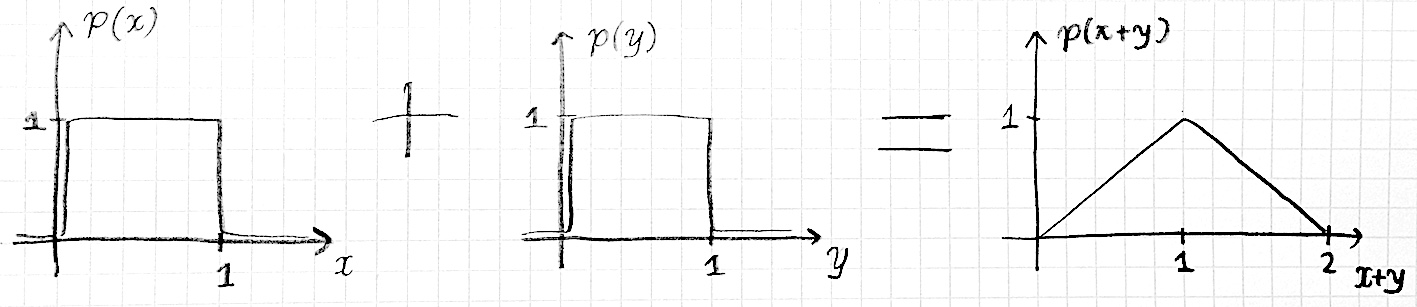
\includegraphics[width=\columnwidth]{somma}
		\caption{Distribuzione della somma di due uniformi.}
	\end{figure}
	$\begin{aligned}[t]
		p(x) &= \chi_{[0,1]}(x) \is \begin{cases}
			1 & x \in [0,1] \\
			0 & \text{altrimenti}
		\end{cases} \\
		p_s(s) &= \int_{-\infty}^{\infty}\de x\, p(x)p(s-x) = \\
		&= \int_{-\infty}^{\infty}\de x\, \chi_{[0,1]}(x)\, \chi_{[0,1]}(s-x) = \\
		&= \int_0^1 \de x\, \chi_{[s-1,s]}(x) = \begin{cases}
			s & s\le1 \\
			2-s & s>1
		\end{cases}.
	\end{aligned}$
\end{solution*}

\begin{exercise}
	Distribuzione di prodotto e rapporto di variabili uniformi in $(0,1)$.
\end{exercise}

\begin{solution}
	\begin{description}
		\item[Prodotto]
			$\begin{aligned}[t]
				p(s) &= \int_{-\infty}^\infty \frac{\de x}{|x|} \chi_{(0,1)}(x)\chi_{(0,1)}\left(\frac sx\right) = \\
				&= \int_0^1 \frac{\de x}{x} \chi_{(s,\infty)}(x) = \\
				&= \begin{cases}
					\int_s^1\frac{\de x}x = -\log s & s \in (0,1) \\
					0 & s \le 0 \vee s \ge 1
				\end{cases}
			\end{aligned}$
		\item[Rapporto]
			$\begin{aligned}[t]
				p(s) &= \int_{-\infty}^\infty \de x\,|x|\,\chi_{(0,1)}(x)\,\chi_{(0,1)}(sx) = \\
				&= \int_0^1 \de x\,x\,\chi_{(0,1/s)}(x) = \\
				&= \begin{cases}
					0 & s \le 0 \\
					\int_0^1 x\de x = \frac12 & 0 < s \le 1 \\
					\int_0^{1/s} x\de x = \frac1{2s^2} & s > 1
				\end{cases}
			\end{aligned}$
	\end{description}
\end{solution}

\begin{exercise}
	Distribuzione di $y=x^2$ con $x$ uniforme in (a) $[0,1]$ o (b) $[-1,1]$.
\end{exercise}

\begin{solution}
	La distribuzione di $y=x^2$ è $1/x$ per la parte pari di $p(x)$ (vedi \autoref{th:stat1d}). Si ottiene
	\begin{enumerate}[(a)]
		\item
			$\displaystyle p(y) = \left.\frac{\chi_{[0,1]}(x) + \chi_{[0,1]}(-x)}{2x}\right|_{x=\sqrt y}
			= \left.\frac{\chi_{[0,1]}(x)}{2x}\right|_{x=\sqrt y}
			= \frac{\chi_{[0,1]}(y)}{2\sqrt y};$
		\item
			$\displaystyle p(y) = \left.\frac{\frac12\chi_{[-1,1]}(x) + \frac12\chi_{[-1,1]}(-x)}{2x}\right|_{x=\sqrt y}
			= \left.\frac{\chi_{[-1,1]}(x)}{2x}\right|_{x=\sqrt y}
			= \frac{\chi_{[0,1]}(y)}{2\sqrt y}.$
	\end{enumerate}
	Il risultato è lo stesso perché la distribuzione~(b) è la parte pari della distribuzione~(a).
\end{solution}
